\documentclass{report}
\usepackage[utf8]{inputenc}

\title{
    Titolo Progetto \\
    \large Applicazioni e Servizi Web
}

\author{Nome Autore - 000725342 \{nome.cognome@unibo.it\}}
\date{01 Gennaio 2020}

\usepackage{natbib}
\usepackage{graphicx}

\begin{document}

\maketitle
\section{Introduzione}
Introduzione \citep{adams1995hitchhiker}

\section{Requisiti}
Descrizione delle caratteristiche e funzionalità che il sistema prevede. 

\section{Design}
Design dell'architettura del sistema e delle interfacce utente.

\begin{figure}[h!]
\centering
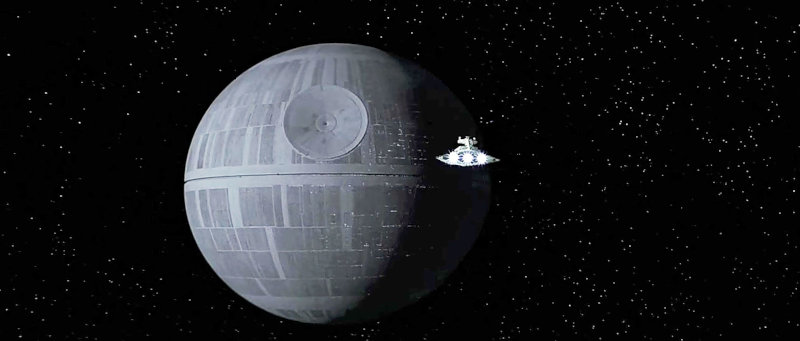
\includegraphics[scale=0.44]{deathStar2.jpg}
\caption{Death Star}
\label{fig:deathstar}
\end{figure}

\section{Tecnologie}
Tecnologie adottate e motivazioni.

\section{Codice}
Solo aspetti rilevanti.

\section{Test}
Test effettuati sul codice e test con utenti.

\section{Deployment}
Rilascio, installazione e messa in funzione.


\section{Conclusioni}
Conclusioni

\bibliographystyle{plain}
\bibliography{references}
\end{document}
